%!TEX root = ../main.tex

\chapter{保拓扑的网格近似算法}
在上一章中我们介绍了现有的四种比较主流的网格简化算法。就简化结果而言,相对复杂的基于内外壳的简化算法不仅能够更好地控制简化误差,而且能够在相同误差下获得更高的简化程度,在相同的简化程度下获得更低的误差。最近Manish Mandad等人将网格重建和带有内外壳的网格简化算法进行了有机地结合,提出了一种新型的鲁棒的保拓扑的网格近似简化算法\cite{isotopic-appro}。与其他基于内外壳的网格简化算法不同,该算法以给定误差空间的内外边界上的采样点为输入,先重建再简化,因此,对原网格的要求更低——只要能通过原网格生成比较好的内外边界采样点如图\ref{fig:iso-appro-robust}。该算法通过空间四面体化,并通过这个四面体网格中线性差值维护一个空间中的误差函数$\epsilon(s)$,来控制简化结果与原模型之间的误差在用户给定的范围内。该算法大致可以分为以下步骤:
\begin{enumerate}[(1)]
  \item 细化,构建误差空间Ω的近似Γ;
  \item 简化误差空间Γ的边界;
  \item 镶嵌 0-等值点;
  \item 简化 0-等值面;
  \item 所有可能的简化。
\end{enumerate}
\begin{figure}[htbp]
    \centering
    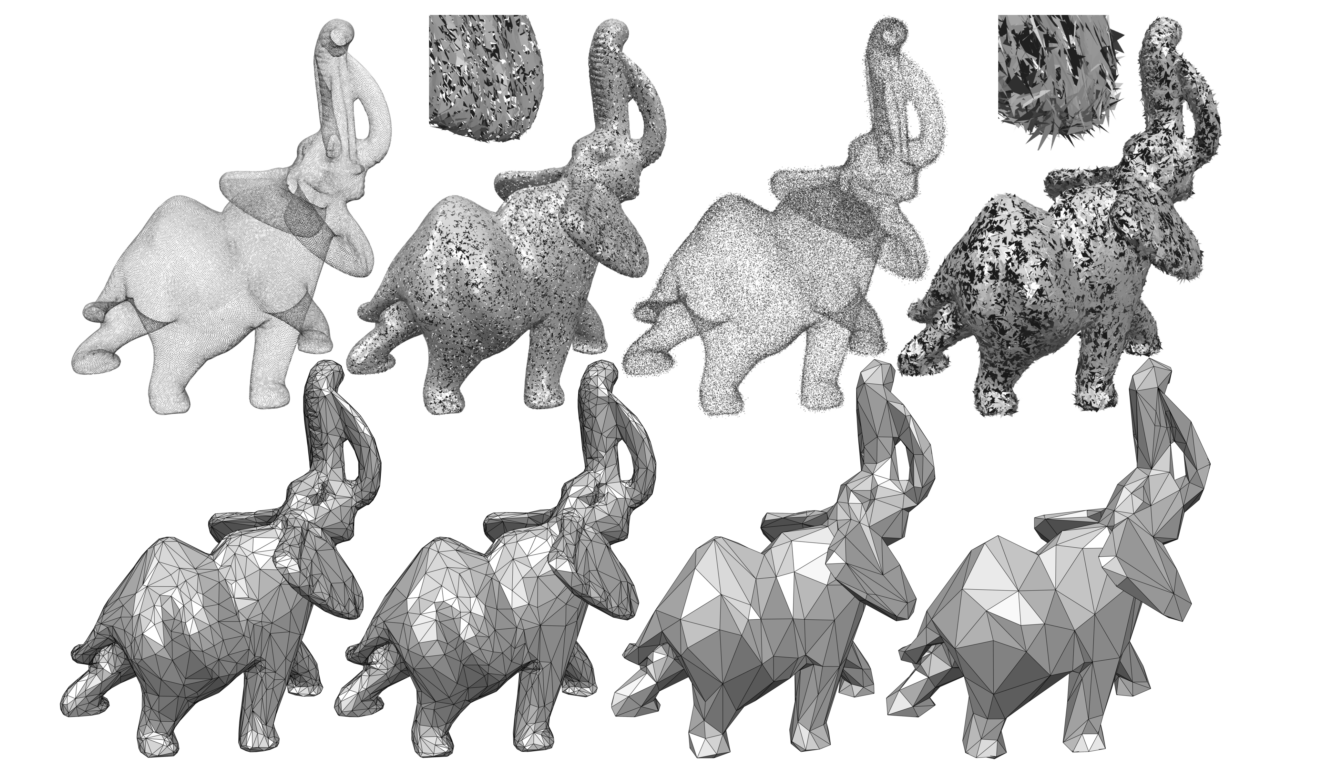
\includegraphics[width=.8\textwidth]{iso_appro_robust.png}
    \caption[保拓扑的网格近似算法的鲁棒性]{保拓扑的网格近似算法能鲁棒地处理带有噪声的输入数据。从左到右分别是顶点集合,带有低噪声的三角面片集合,带有高噪声的顶点集合以及带有高噪声的三角面片集合。第二行是对这些数据的简化结果,图引用自\cite{isotopic-appro}}
    \label{fig:iso-appro-robust}
\end{figure}

\section{细化,构建误差空间Ω的近似Γ}
对于给定的误差空间为$\Omega$,算法以对误差空间$\Omega$的边界$\partial \Omega$上的一个密度为$\sigma$的采样(以每个采样点为圆心,以$\sigma$为半径的圆球,能够覆盖整个$\partial \Omega$)所得到的采样点集合S作为输入。算法假定这个误差空间只有两个边界,内边界和外边界,定义$S_0$为内边界采样点,$S_1$为外边界采样点,$S_{bs}$为包围球上的采样点。在S上定义一个参照函数:
\begin{equation}
  \begin{split}
    F(s) &= -1, s\in S_0\\
    F(s) &= +1, s\in S_1\\
    F(s) &= +1, s\in S_{bs}
  \end{split}
\end{equation}
然后以$\Omega$的包围球上的采样点$S_{bs}$作为初始化顶点,做一个四面体化,得到四面体网格$\tau$。在$\tau$上针对每一个四面体维护一个线性差值函数:
\begin{equation}
  f(s) = \sum_{i=0}^3 w_iF(s_i), s\in tet(s_0, s_1, s_2, s_3), s_i \in \tau
  \label{eq:linear-interpolation}
\end{equation}
这里,$tet(s_0, s_1, s_2, s_3)$是由这四个顶点所构成的四面体,$w_i$是顶点s在这个四面体上的重心坐标分量。所谓重心坐标是指对于四面体$tet(s_0, s_1, s_2, s_3)$中的一个顶点s,我们可以通过这四个点的加权来得到s的坐标值即:
\begin{equation}
  \begin{split}
  \sum_{i=0}^3 w_i s_i &= s\\
  \sum_{i=0}^3 w_i &= 1
  \end{split}
  \label{eq:err-constraint}
\end{equation}
这样,我们就可以得到每一个内外壳上的采样点的对应函数值,定义所有$f(s)=0$的点的集合为$\mathcal{Z}$即0-等值面,而当内外采样点的$f(s)$函数值与参照函数$F(s)$的函数值相差不超过1的时候,这个0-等值面$\mathcal{Z}$能够正确地将$S_0$和$S_1$的采样点区分开,也即0-等值面不会超越误差空间(如图\ref{fig:isotopic-classification})。因此,在采样点S上定义一个误差函数:
\begin{equation}
  \epsilon(s) = \lVert f(s)-F(s) \rVert
\end{equation}
从而误差约束条件转化为:
\begin{equation}
  \forall s \in S, \epsilon(s)<1
\end{equation}

\begin{figure}[htbp]
    \centering
    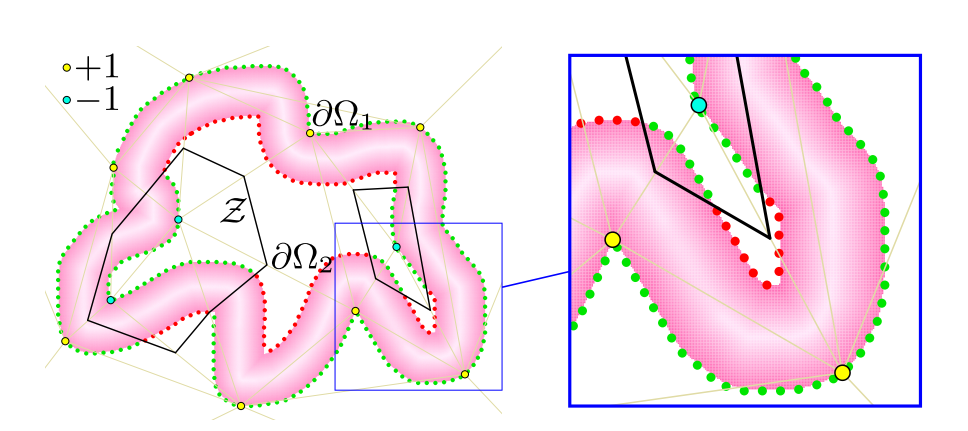
\includegraphics[width=.7\textwidth]{classification.png}
    \caption[0-等值面区分误差边界采样点]{图中绿色的点已经被0-等值面正确地分开,而红色的点未被正确地分开,图来自\cite{isotopic-appro}}
    \label{fig:isotopic-classification}
\end{figure}

\begin{figure}[htbp]
    \centering
    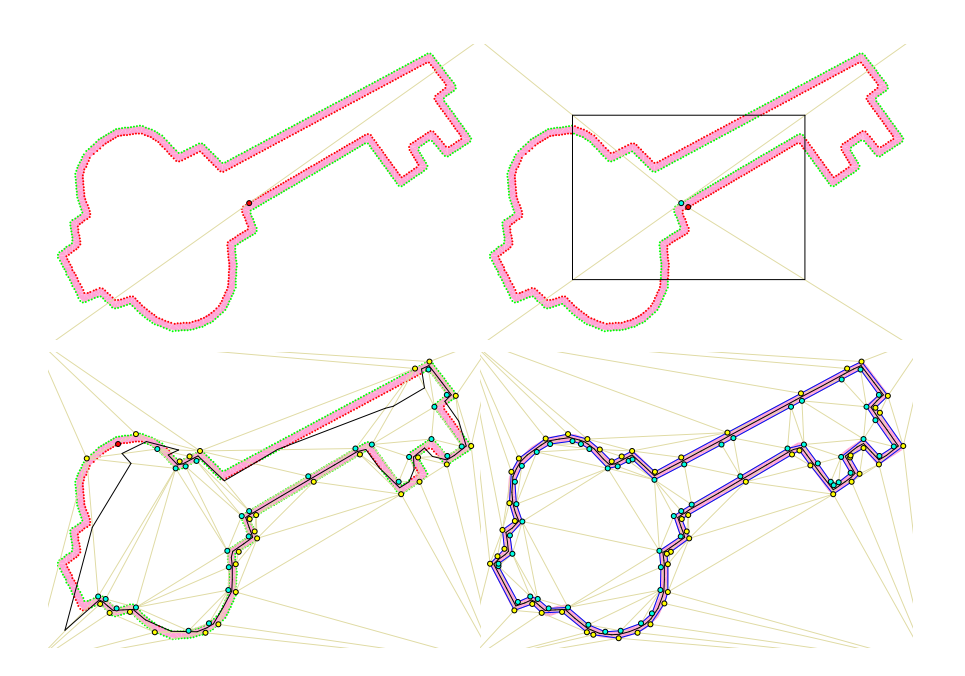
\includegraphics[width=.7\textwidth]{refine.png}
    \caption[细化过程]{细化的过程——逐渐地加入采样点直到所有的采样点能够被0-等值面正确地区分开,图来自\cite{isotopic-appro}}
    \label{fig:refine}
\end{figure}

\par 在细化阶段基本思路是:使用贪心的策略不断地选取$s \in S,\epsilon(s)$最大的顶点加入到$\tau$中,并重做四面体化直到直到$\tau$达到这个约束条件(如图\ref{fig:refine})。不过为了保持法向的质量,尽可能避免简化后的网格可能会出现法向翻转的问题(如图\ref{fig:normal-cond}),需要添加一个额外的法向约束条件:在每一个四面体上定义的线型差值函数不仅能够正确地区分在该四面体内的S中的采样点,而且当该四面体缩小到一个比例$\alpha$后,该线性差值函数也能够区分内外壳上离缩小的四面体的四个顶点最近的采样点。在整个细化的过程中,依次判断误差约束条件,以及法向约束条件是否得到满足。
\begin{figure}[htbp]
    \centering
    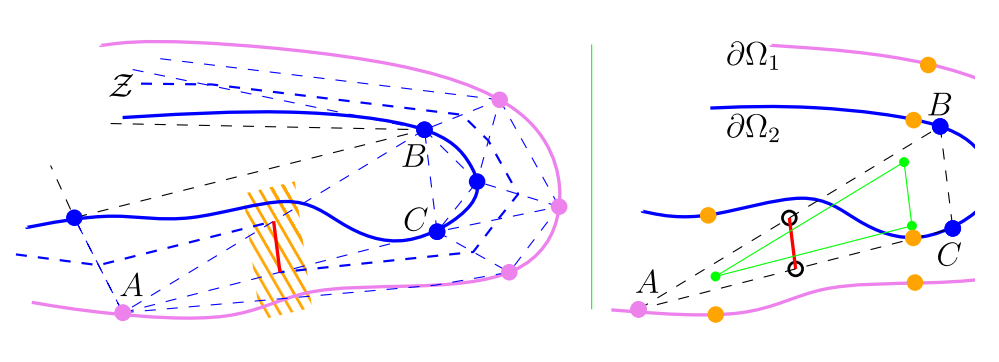
\includegraphics[width=.7\textwidth]{normal_cond.png}
    \caption[法向约束条件]{由于三角化不合理导致的法向不合理的情况(左图红色边)。右图是对法向是否合理的一个检测,红色的边并不能将绿色三角形($\triangle ABC$缩小一定比例之后的三角形)的三个顶点最近的内外壳采样点(橘黄色的顶点)正确地划分开,图来自\cite{isotopic-appro}}
    \label{fig:normal-cond}
\end{figure}
为了得到一个质量相对较好的四面体网格$\tau$(尽量避免细长的四面体出现),使用3D Delaunnay三角化来为空间中的顶点构建四面体网格。对于$\mathbb{R}^3$上的顶点集合S,其3D Delaunay三角化$(DT)$的结果$D(S)$是一个满足对于任意一个$D(S)$上的四面体,没有其他顶点落在它的外接球内部(如图\ref{fig:2d-delaunay})。对于$S$上的一个3D三角化$\tau$,对于一个三角面片$f \in \tau$,若$f$与由其所构成的四面体的任一外接球中的顶点均没有边相连,那么我们所这个三角面片f是局部Delaunay的。如果$\tau$中的所有三角面片都是局部Delaunay的,那么$\tau \equiv D(S)$。3D Delaunnay三角化的一个重要特点是能够最小化四面体网格中四面体的最大外接球。因此,3D Delaunay三角化能够尽可能避免一些狭长的四面体的出现,获得质量较好地四面体网格。在细化结束后,就得到了一个原误差空间$\Omega$的近似$\Gamma$。也得益于3D Delaunay三角化,对于不满足法向约束条件的四面体,可以选取离该四面体外接球球心最近的采样点加入到四面体网格$\tau$中,然后更新四面体网格$\tau$。由于采用3D Delaunay三角化的性质,加入这样的点会破坏原不满足法向约束条件的四面体(在新的题网格$\tau$中,这四个点不构成一个四面体),从而达到了消除不满足法向约束条件的四面体的功能。
\begin{figure}[htbp]
    \centering
    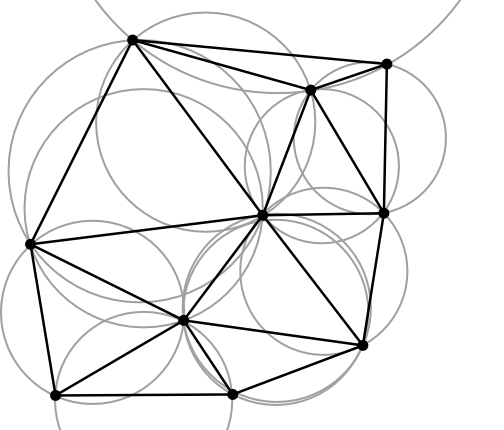
\includegraphics[width=.5\textwidth]{2d_delaunay.png}
    \caption[2D Delaunay]{2D上的Delaunnay三角化示意图,引用自\cite{delaunay-wiki}}
    \label{fig:2d-delaunay}
\end{figure}

\section{误差边界$\partial \Gamma$的简化}
在初始化得到了一个满足误差控制要求的四面体网格$\tau$,通过消除这个近似误差空间$\Gamma$的边界$\partial \Gamma$上的边来简化$\partial \Gamma$。首先需要保证简化过后的四面体网格$\tau$仍然是一个有效的四面体网格:
\begin{enumerate}[(1)]
  \item 四面体网格的拓扑结构是有效的(保证不会出现不属于任何四面体的面等);
  \item 四面体网格是包围球空间的一个有效的填充,即不存在相互交叉的四面体。
\end{enumerate}
为了保证简化后的τ足第一个条件,需要保证我们消除的边需满足Dey等人提出的Link Condition\cite{link-cond},而对于第二个条件需要使得消除的边的合并点落在这条边的Kernel Region中。除了上述两个基本的条件外,还需要保简化满足误差约束条件\eqref{eq:err-constraint},以及为了维持法向质量所加的法向约束。

\subsection{Link Condition}
借鉴Dey等人对保持拓扑有效性的消边的研究\cite{link-cond},在$\tau$上做消边操作时,需要判断该边是否满足Link Condition。一个由k+1个独立的点构成的凸包$\sigma$,被称为k-simplex,比如 0-simplex ——点,1-simplex ——线段。$\sigma$上的一个非空子集t,称为$\sigma$的face,而相对的$\sigma$是t的coface。定义由有限个k-simplex构成的一个集合$\mathcal{K}$,称为simplical complex。这里的四面体网格$\tau$就是这样的一个simplical complex。假设B是一个simplical complex $\mathcal{K}$上的一个子集,则定义B的closure ——$\overline{B}$(如图\ref{fig:closure}),为包含B中所有face的最小simplical complex。而B的star ——$St B$(如图\ref{fig:star}),定义为包含B中每一个simplex的star的并集,一个simpex的star即为该simplex的coface。而Lk(B):$Lk B = \overline{St B} - St \overline{B}$(如图\ref{fig:link})。\par

\begin{figure}[htbp]
    \centering
    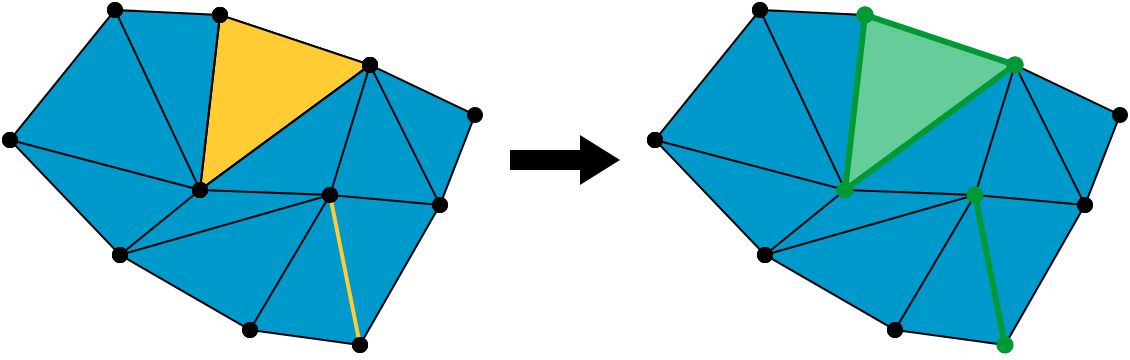
\includegraphics[width=.7\textwidth]{simplicial_complex_closure.png}
    \caption[2D closure]{2D三角网格上的closure示意图,图引用自\cite{simplicial-complex}}
    \label{fig:closure}
\end{figure}
\begin{figure}[htbp]
    \centering
    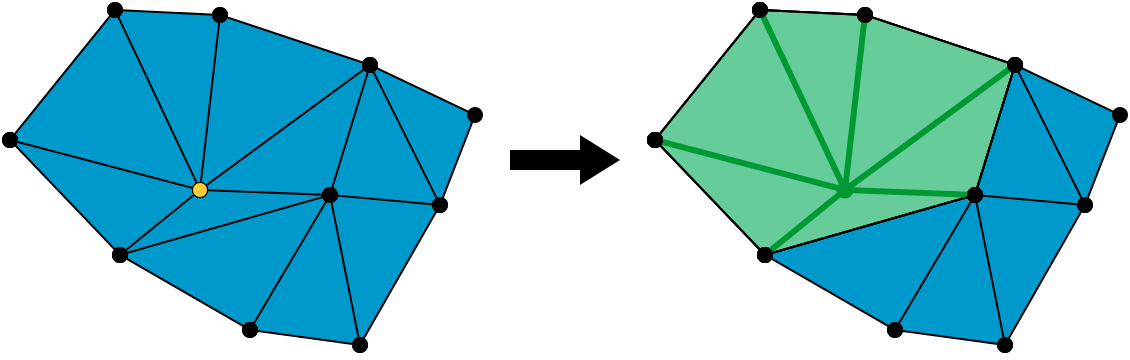
\includegraphics[width=.7\textwidth]{simplicial_complex_star.png}
    \caption[2D star]{2D三角网格上的star示意图,图引用自\cite{simplicial-complex}}
    \label{fig:star}
\end{figure}
\begin{figure}[htbp]
    \centering
    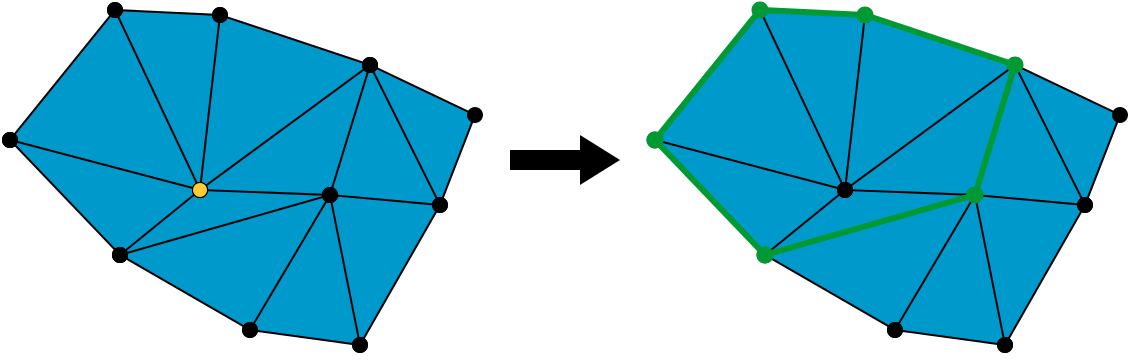
\includegraphics[width=.7\textwidth]{simplicial_complex_link.png}
    \caption[2D link]{2D三角网格上的link示意图,图引用自\cite{simplicial-complex}}
    \label{fig:link}
\end{figure}
从而边AB上的Link Condition定义为$Lk(A) \cap Lk(B) = LK(AB)$。从Link Condition中我们可以直观地发现,对于2D空间中的一个点A其Lk(A)为顶点A的一环邻域的边界上的顶点和边,而$Lk(AB)$则是包含边AB的三角形的另一个顶点,边AB的Link Condition是否满足等价于A和B各自一环邻域的边界不能相交于一条边,否则AB合并之后该边将成为一条孤立的边(不属于任何三角形,如图\ref{fig:2d-link-cond})。类似的对于3D空间上AB的Link Condition是否满足等价于A和B各自的一环邻域的边界不能相交于一个面,否则AB合并之后该面将成为一个孤立的面(不属于任何四面体,如图\ref{fig:3d-link-cond})。
\begin{figure}[htbp]
    \centering
    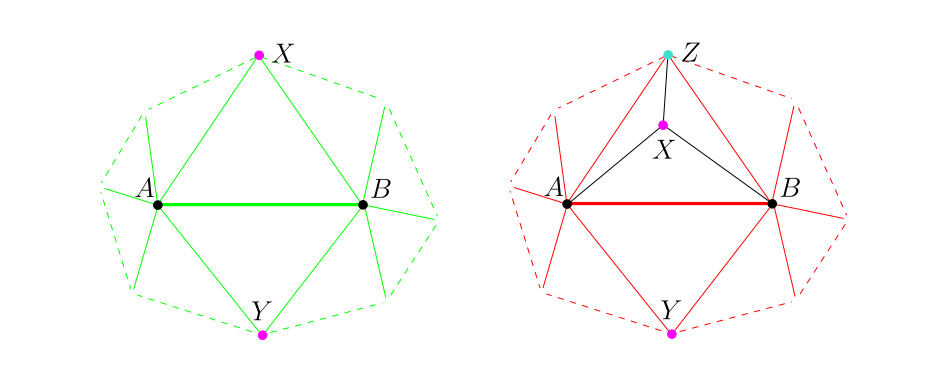
\includegraphics[width=.7\textwidth]{2d_link_cond.png}
    \caption[2D Link Condition]{2D三角网格上的Link Condition示意图,对于边AB,左图满足Link Condition,右图不满足Link Condition,图引用自\cite{isotopic-appro}}
    \label{fig:2d-link-cond}
\end{figure}
\begin{figure}[htbp]
    \centering
    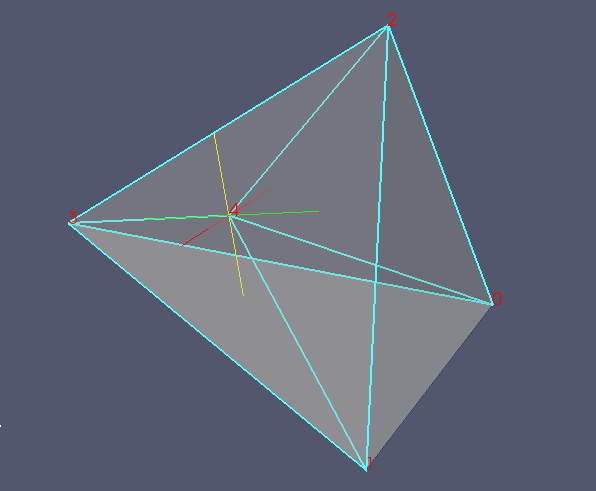
\includegraphics[width=.5\textwidth]{3d_link_cond.png}
    \caption[3D Link Condition]{3D三角网格上的Link Condition示意图,顶点1和3不能被合并,若顶点1和3合并,则会出现一个不属于任何四面体的三角面片024}
    \label{fig:3d-link-cond}
\end{figure}

\subsection{Kernel Region}
为了保证消边之后$\tau$仍然是包围球空间的一个有效填充,即不会产生四面体相互交叉的情况,需要保证得新生成的四面体是边PQ——环邻域的空间(由包含P或Q的四面体构成的空间)的有效填充。因此,PQ的合并点必须落在PQ的邻域空间的边界的每一个三角形内侧。我们定义该空间为边PQ的Kernel Region——$K_\tau(PQ)$(如图\ref{fig:kernel-region}是2D的Kernel Region示意图)。
\begin{figure}[htbp]
    \centering
    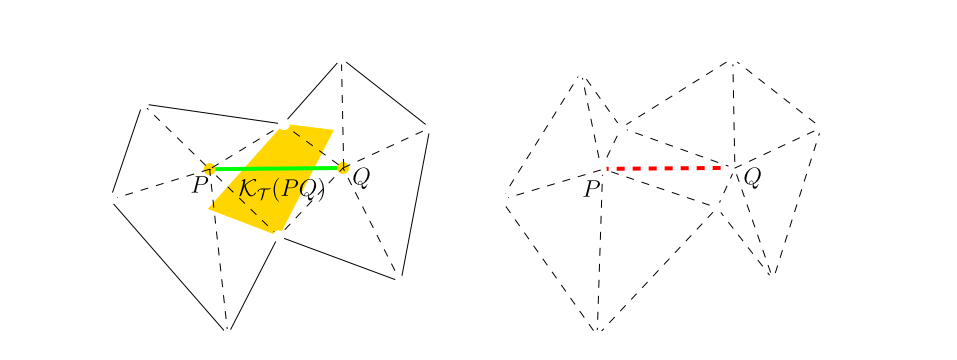
\includegraphics[width=.8\textwidth]{kernel_region.png}
    \caption[2D Kernel Region]{在二维中一条边的PQ的Kernel Region为PQ的一环邻域的三角面片边界上,每一条边所对应的直线的内侧(PQ这一侧)的交集,图引用自\cite{isotopic-appro}}
    \label{fig:kernel-region}
\end{figure}
\par 在对$\partial \Gamma$进行消边时,从内外壳的采样点中选取合并点。除了需要满足保持四面体网格$\tau$的有效性外,还需要保证满足误差控制条件$\forall s \in S, \delta(s) < 1$。因此,需要对$K_\tau (PQ) \cap S$中所有的点,逐个判断若合并到该点后,新生成的四面体空间中所有的采样点是否满足$\delta(s) < 1$,若满足则合并到这个点,否则继续尝试下一个点。若$K_\tau (PQ) \cup S$所有的点都无法保持$\delta(s) < 1$这个条件,则放弃消除这条边。和其他简化算法类似,为了找到一个更优的合并点的位置,使得误差更小,可以对所有的采样点根据其到PQ的2环邻域的每一个0-等值三角形所在平面的距离平方和由小到大做一个优先级排序。
\section{0-等值面的生成}
当误差边界$\partial \Gamma$简化完成之后,将$\tau$中每一条由连接内外边界$(\partial \Gamma_0, \partial \Gamma_1)$的边的中点——0-等值点嵌入到这个四面体中并细分这个四面体网格,从而得到由0-等值点构成的0-等值面$\mathcal{Ζ}$,现在$\mathcal{Z}$是在误差空间$\Omega$中原网格的一个保拓扑的近似(如图\ref{fig:mutual-tessellation})。
\begin{figure}[htbp]
    \centering
    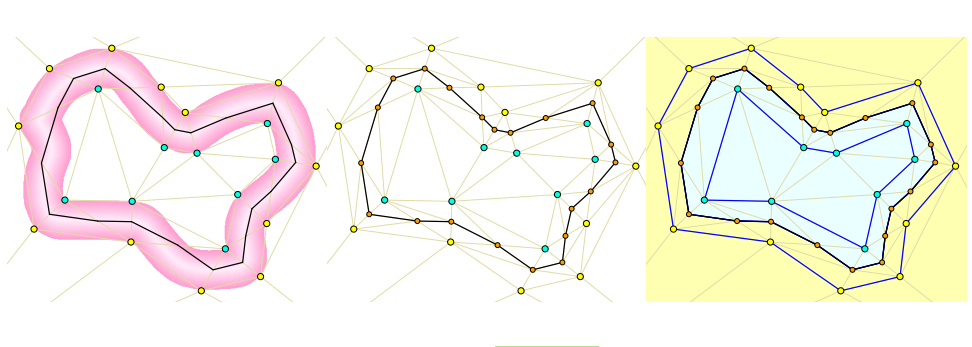
\includegraphics[width=.8\textwidth]{mutual_tessellation.png}
    \caption[Mutual tessellation]{在二维上的0-等值点嵌入:左图为在0-等值点嵌入之前;中间图为0-等值点嵌入之后;右图显示了$\partial \Gamma$的边界线蓝色线,以及0-等值线黑色线,以及函数$f(s)$的取值情况,黄色区域$f(s) > 0$,淡蓝色区域$f(s) < 1$,图引用自\cite{isotopic-appro}}
    \label{fig:mutual-tessellation}
\end{figure}

\section{所有可能的简化}
由于$\Gamma$是原误差空间$\Omega$的一个简化近似,因此,0-等值面的简化可能无法充分利用$\Omega$的空间(如图\ref{fig:tol-small})。为了尽可能充分地利用误差空间,可以通过尝试消除由0-等值点或边界上的点构成的边来调整0-等值点的位置,并扩大0-等值面上的边的Kernel Region,从而达到进一步简化的目的(如图\ref{fig:all-edges-collapse})。当所有简化都结束之后,最终的0-等值面就是我们的简化结果。

\begin{figure}[htbp]
    \centering
    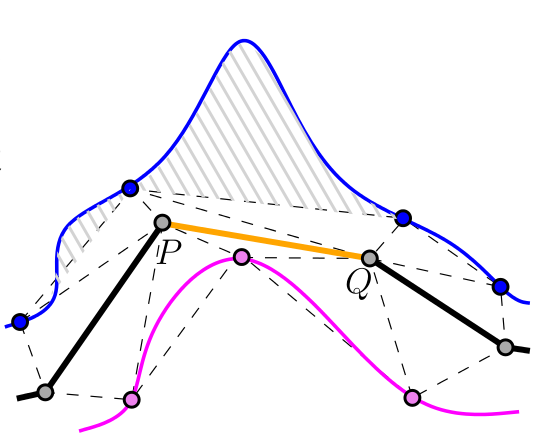
\includegraphics[width=.5\textwidth]{tol_small.png}
    \caption[无法利用的误差空间]{图中阴影部分空间无被充分利用起来,图引用自\cite{isotopic-appro}}
    \label{fig:tol-small}
\end{figure}

\begin{figure}[htbp]
    \centering
    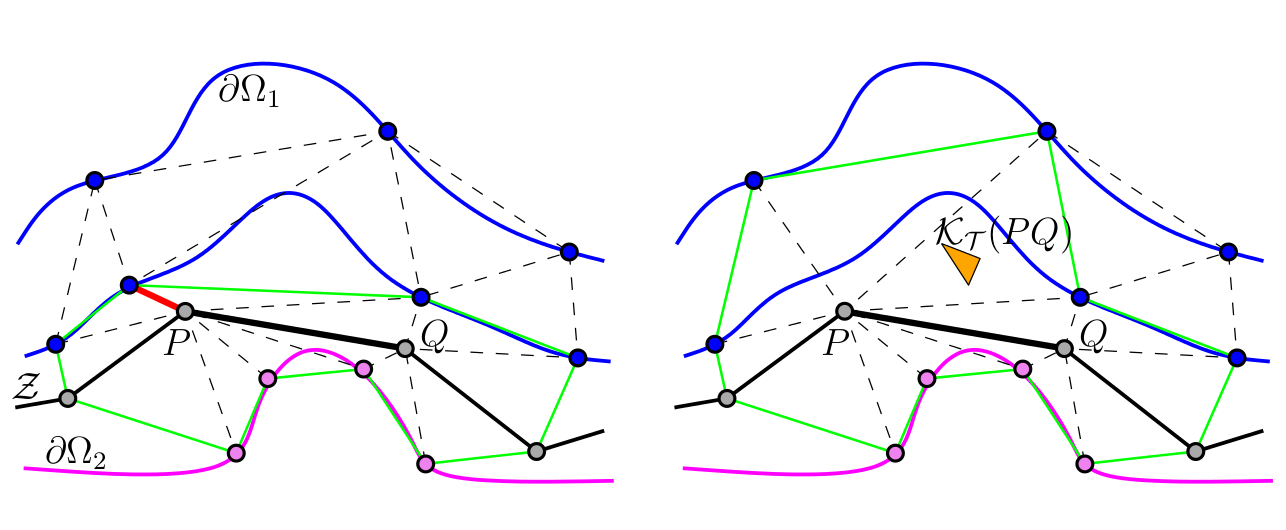
\includegraphics[width=.9\textwidth]{zb_collapse.png}
    \caption[所有可能的边的消除]{通过消除所有可能的边来进一步简化网格。左图中边PQ由于Kernel Region为空而无法消除,在右图中通过消除左图中的红色边,PQ的Kernel Region变为橙色的区域(不为空),从而增大了PQ消除的可能性。图引用自\cite{isotopic-appro}}
    \label{fig:all-edges-collapse}
\end{figure}

\section{本章小结}
本章详细介绍了Manish Mandad等人提出的保拓扑的网格近似算法\cite{isotopic-appro}。本章首先简述了该算法的其特点,并详细介绍了其主要步骤。该算法以误差空间$\Omega$的边界上的采样点S作为输入。以S的包围球上的顶点初始化顶点,利用 3D Delaunay三角化建立起一个四面体网格$\tau$,并在这个四面体网格上维护一个误差函数$\epsilon(s)$,贪心地从S中选取误差最大的顶点插入到$\tau$中,直到S中所有点的误差不超过1。然后在保持$\tau$有效、保持误差约束和保持法向约束条件的前提下、通过简化误差边界,得到一个更加稀疏的误差空间$\Omega$的近似。再通过嵌入0-等值点得到显式的0-等值面。最后通过简化0-等值面和所有可能的简化得到最终的简化结果。

